\section{Exploratory factor analysis}
\frame{\sectionpage}


\begin{frame}[fragile]{Principal components and factor analysis}

  \begin{itemize}
  \item Principal components: 
    \begin{itemize}
    \item Purely mathematical.
    \item Find eigenvalues, eigenvectors of correlation matrix.
    \item No testing whether observed components reproducible, or even probability model behind it.
    \end{itemize}
  \item Factor analysis: 
    \begin{itemize}
    \item some way towards fixing this (get test of appropriateness)
    \item In factor analysis, each variable modelled as: ``common factor'' (eg. verbal ability) and ``specific factor'' (left over).
    \item Choose the common factors to ``best'' reproduce pattern seen in correlation matrix.
    \item Iterative procedure, different answer from principal components.
    \end{itemize}

  \end{itemize}

\end{frame}

\begin{frame}[fragile]{Example}

  \begin{itemize}
  \item 
145 children given 5 tests, called PARA, SENT, WORD, ADD and DOTS. 3 linguistic tasks (paragraph comprehension, sentence completion  and word meaning), 2 mathematical ones (addition and counting dots).
\item Correlation matrix of scores on the tests:

\begin{verbatim}
para 1     0.722 0.714 0.203 0.095
sent 0.722 1     0.685 0.246 0.181
word 0.714 0.685 1     0.170 0.113
add  0.203 0.246 0.170 1     0.585
dots 0.095 0.181 0.113 0.585 1
\end{verbatim}

\item Is there small number of underlying ``constructs'' (unobservable) that explains this pattern of correlations?


  \end{itemize}
  
\end{frame}

\begin{frame}[fragile]{To start: principal components}

Using correlation matrix:

\begin{knitrout}
\definecolor{shadecolor}{rgb}{0.969, 0.969, 0.969}\color{fgcolor}\begin{kframe}
\begin{alltt}
\hlstd{kids}\hlkwb{=}\hlkwd{read.table}\hlstd{(}\hlstr{"rex2.txt"}\hlstd{,}\hlkwc{header}\hlstd{=T)}
\hlstd{km}\hlkwb{=}\hlkwd{as.matrix}\hlstd{(kids)}
\hlstd{kids.pc}\hlkwb{=}\hlkwd{princomp}\hlstd{(}\hlkwc{covmat}\hlstd{=km)}
\end{alltt}
\end{kframe}
\end{knitrout}

\end{frame}

\begin{frame}[fragile]{Scree plot}
   
\begin{knitrout}
\definecolor{shadecolor}{rgb}{0.969, 0.969, 0.969}\color{fgcolor}\begin{kframe}
\begin{alltt}
\hlkwd{plot}\hlstd{(kids.pc}\hlopt{$}\hlstd{sdev}\hlopt{^}\hlnum{2}\hlstd{,}\hlkwc{type}\hlstd{=}\hlstr{"b"}\hlstd{,}\hlkwc{ylab}\hlstd{=}\hlstr{"Eigenvalue"}\hlstd{)}
\end{alltt}
\end{kframe}
\includegraphics[width=\maxwidth]{figure/unnamed-chunk-1-1} 

\end{knitrout}
  
%  \includegraphics[height=\textheight]{bFactor-kids-scree}
  
\end{frame}

\begin{frame}[fragile]{Principal component results}
  
  \begin{itemize}
  \item Need 2 components.
  \item Loadings:
{\footnotesize
\begin{knitrout}
\definecolor{shadecolor}{rgb}{0.969, 0.969, 0.969}\color{fgcolor}\begin{kframe}
\begin{alltt}
\hlstd{kids.pc}\hlopt{$}\hlstd{loadings}
\end{alltt}
\begin{verbatim}
## 
## Loadings:
##      Comp.1 Comp.2 Comp.3 Comp.4 Comp.5
## para -0.534 -0.245 -0.114         0.795
## sent -0.542 -0.164        -0.660 -0.489
## word -0.523 -0.247  0.144  0.738 -0.316
## add  -0.297  0.627 -0.707              
## dots -0.241  0.678  0.680         0.143
## 
##                Comp.1 Comp.2 Comp.3 Comp.4 Comp.5
## SS loadings       1.0    1.0    1.0    1.0    1.0
## Proportion Var    0.2    0.2    0.2    0.2    0.2
## Cumulative Var    0.2    0.4    0.6    0.8    1.0
\end{verbatim}
\end{kframe}
\end{knitrout}
}
%$
\item First component has a bit of everything, though especially the
  first three tests.
\item Second component rather more clearly \texttt{add} and \texttt{dots}.
\item No scores, plots since no actual data.
  
  \end{itemize}
  
  
  
\end{frame}


\begin{frame}[fragile]{Factor analysis}
  
  \begin{itemize}
  \item Specify number of factors first, get solution with exactly
    that many factors.
  \item Includes hypothesis test, need to specify how many children
    wrote the tests.
  \item Works from correlation matrix via \texttt{covmat} or actual
    data, like \texttt{princomp}.
  \item Introduces extra feature, \emph{rotation}, to make
    interpretation of loadings (factor-variable relation) easier.
  \end{itemize}
  
\end{frame}

\begin{frame}[fragile]{Factor analysis for the kids data}

  \begin{itemize}
  \item Create ``covariance list'' to include number of children who
    wrote the tests.
  \item Feed this into \texttt{factanal}, specifying how many factors (2).
  \end{itemize}
  
\begin{knitrout}
\definecolor{shadecolor}{rgb}{0.969, 0.969, 0.969}\color{fgcolor}\begin{kframe}
\begin{alltt}
\hlstd{km2}\hlkwb{=}\hlkwd{list}\hlstd{(}\hlkwc{cov}\hlstd{=km,}\hlkwc{n.obs}\hlstd{=}\hlnum{145}\hlstd{)}
\hlstd{kids.f2}\hlkwb{=}\hlkwd{factanal}\hlstd{(}\hlkwc{factors}\hlstd{=}\hlnum{2}\hlstd{,}\hlkwc{covmat}\hlstd{=km2)}
\end{alltt}
\end{kframe}
\end{knitrout}

\end{frame}

\begin{frame}[fragile]{Uniquenesses}

\begin{knitrout}
\definecolor{shadecolor}{rgb}{0.969, 0.969, 0.969}\color{fgcolor}\begin{kframe}
\begin{alltt}
\hlstd{kids.f2}\hlopt{$}\hlstd{uniquenesses}
\end{alltt}
\begin{verbatim}
##      para      sent      word       add      dots 
## 0.2424457 0.2997349 0.3272312 0.5743568 0.1554076
\end{verbatim}
\end{kframe}
\end{knitrout}
%$

  \begin{itemize}
  \item Uniquenesses say how ``unique'' a variable is (size of
    specific factor). Small
    uniqueness means that the variable is summarized by a factor (good).
    
  \item Mildly worried by how large \texttt{add}'s uniqueness is.
  \item Also see ``communality'' for this, where \emph{large} is good.
  \end{itemize}
  
\end{frame}

\begin{frame}[fragile]{Loadings}

  \begin{minipage}[t]{0.58\linewidth}
    {\small
\begin{knitrout}
\definecolor{shadecolor}{rgb}{0.969, 0.969, 0.969}\color{fgcolor}\begin{kframe}
\begin{alltt}
\hlstd{kids.f2}\hlopt{$}\hlstd{loadings}
\end{alltt}
\begin{verbatim}
## 
## Loadings:
##      Factor1 Factor2
## para 0.867          
## sent 0.820   0.166  
## word 0.816          
## add  0.167   0.631  
## dots         0.918  
## 
##                Factor1 Factor2
## SS loadings      2.119   1.282
## Proportion Var   0.424   0.256
## Cumulative Var   0.424   0.680
\end{verbatim}
\end{kframe}
\end{knitrout}
}

%$
  \end{minipage}
  \begin{minipage}[t]{0.40\linewidth}
  \begin{itemize}
  \item Loadings show how each factor depends on variables. Blanks
    indicate ``small'', less than 0.1.
  \item Factor 1 clearly the ``linguistic'' tasks, factor 2 clearly
    the ``mathematical'' ones.
  \item Two factors together explain 68\% of variability (like
    regression R-squared).
  \end{itemize}    
  \end{minipage}
\end{frame}


\begin{frame}[fragile]{Are 2 factors enough?}
  
\begin{knitrout}
\definecolor{shadecolor}{rgb}{0.969, 0.969, 0.969}\color{fgcolor}\begin{kframe}
\begin{alltt}
\hlstd{kids.f2}\hlopt{$}\hlstd{STATISTIC}
\end{alltt}
\begin{verbatim}
## objective 
## 0.5810578
\end{verbatim}
\begin{alltt}
\hlstd{kids.f2}\hlopt{$}\hlstd{dof}
\end{alltt}
\begin{verbatim}
## [1] 1
\end{verbatim}
\begin{alltt}
\hlstd{kids.f2}\hlopt{$}\hlstd{PVAL}
\end{alltt}
\begin{verbatim}
## objective 
##  0.445898
\end{verbatim}
\end{kframe}
\end{knitrout}

P-value not small, so 2 factors OK.
  
\end{frame}

\begin{frame}[fragile]{1 factor}

\begin{knitrout}
\definecolor{shadecolor}{rgb}{0.969, 0.969, 0.969}\color{fgcolor}\begin{kframe}
\begin{alltt}
\hlstd{kids.f1}\hlkwb{=}\hlkwd{factanal}\hlstd{(}\hlkwc{factors}\hlstd{=}\hlnum{1}\hlstd{,}\hlkwc{covmat}\hlstd{=km2)}
\hlstd{kids.f1}\hlopt{$}\hlstd{STATISTIC}
\end{alltt}
\begin{verbatim}
## objective 
##  58.16534
\end{verbatim}
\begin{alltt}
\hlstd{kids.f1}\hlopt{$}\hlstd{dof}
\end{alltt}
\begin{verbatim}
## [1] 5
\end{verbatim}
\begin{alltt}
\hlstd{kids.f1}\hlopt{$}\hlstd{PVAL}
\end{alltt}
\begin{verbatim}
##    objective 
## 2.907856e-11
\end{verbatim}
\end{kframe}
\end{knitrout}

1 factor rejected (P-value small). Definitely need more than 1.
  
\end{frame}

\begin{frame}[fragile]{Track running records revisited}
  
    \includegraphics[height=\textheight]{bPrincomp-biplot}

\end{frame}

\begin{frame}{Benefit of rotation}
  
  \begin{itemize}
  \item 100m and marathon arrows almost perpendicular, but components
    don't match anything much:
    \begin{itemize}
    \item sprinting: top left and bottom right
    \item distance running: bottom left and top right.
    \end{itemize}
  \item Can we arrange things so that components (factors) correspond
    to something meaningful?
  \end{itemize}
  
\end{frame}

\begin{frame}[fragile]{Track records by factor analysis}

  Obtain factor scores (have actual data):
  
\begin{knitrout}
\definecolor{shadecolor}{rgb}{0.969, 0.969, 0.969}\color{fgcolor}\begin{kframe}
\begin{alltt}
\hlstd{track}\hlkwb{=}\hlkwd{read.table}\hlstd{(}\hlstr{"men_track_field.txt"}\hlstd{,}\hlkwc{header}\hlstd{=T)}
\hlstd{track.f}\hlkwb{=}\hlkwd{factanal}\hlstd{(track[,}\hlopt{-}\hlnum{9}\hlstd{],}\hlnum{2}\hlstd{,}\hlkwc{scores}\hlstd{=}\hlstr{"r"}\hlstd{)}
\end{alltt}
\end{kframe}
\end{knitrout}
  
\end{frame}

\begin{frame}[fragile]{Track data biplot}
  
\begin{knitrout}
\definecolor{shadecolor}{rgb}{0.969, 0.969, 0.969}\color{fgcolor}\begin{kframe}
\begin{alltt}
\hlkwd{biplot}\hlstd{(track.f}\hlopt{$}\hlstd{scores,track.f}\hlopt{$}\hlstd{loadings,}\hlkwc{xlabs}\hlstd{=track[,}\hlnum{9}\hlstd{])}
\end{alltt}
\end{kframe}
\includegraphics[width=\maxwidth]{figure/siracusa-1} 

\end{knitrout}
  
  % \includegraphics[height=\textheight]{bFactor-track-factor-biplot}
  
\end{frame}

\begin{frame}[fragile]{Comments}
  
  \begin{itemize}
  \item This time 100m ``up'' (factor 2), marathon ``right'' (factor 1).
  \item Countries most negative on factor 2 good at sprinting.
  \item Countries most negative on factor 1 good at distance running.
  \end{itemize}
  
\end{frame}

\begin{frame}[fragile]{Rotated factor loadings}

  {\small
\begin{knitrout}
\definecolor{shadecolor}{rgb}{0.969, 0.969, 0.969}\color{fgcolor}\begin{kframe}
\begin{alltt}
\hlstd{track.f}\hlopt{$}\hlstd{loadings}
\end{alltt}
\begin{verbatim}
## 
## Loadings:
##          Factor1 Factor2
## m100     0.291   0.914  
## m200     0.382   0.882  
## m400     0.543   0.744  
## m800     0.691   0.622  
## m1500    0.799   0.530  
## m5000    0.901   0.394  
## m10000   0.907   0.399  
## marathon 0.915   0.278  
## 
##                Factor1 Factor2
## SS loadings      4.112   3.225
## Proportion Var   0.514   0.403
## Cumulative Var   0.514   0.917
\end{verbatim}
\end{kframe}
\end{knitrout}
  }
  
\end{frame}

\begin{frame}[fragile]{Which countries are good at sprinting or
    distance running?}
  
\begin{knitrout}
\definecolor{shadecolor}{rgb}{0.969, 0.969, 0.969}\color{fgcolor}\begin{kframe}
\begin{alltt}
\hlstd{good.sprint}\hlkwb{=}\hlstd{track.f}\hlopt{$}\hlstd{scores[,}\hlnum{2}\hlstd{]}\hlopt{<}\hlstd{(}\hlopt{-}\hlnum{1}\hlstd{)}
\hlstd{track[good.sprint,}\hlnum{9}\hlstd{]}
\end{alltt}
\begin{verbatim}
## [1] bm dr uk it us ru
## 55 Levels: ar at au be bm br bu ca ch ck cl cn co cr cz dee dew dk ... ws
\end{verbatim}
\begin{alltt}
\hlstd{good.distance}\hlkwb{=}\hlstd{track.f}\hlopt{$}\hlstd{scores[,}\hlnum{1}\hlstd{]}\hlopt{<}\hlstd{(}\hlopt{-}\hlnum{0.8}\hlstd{)}
\hlstd{track[good.distance,}\hlnum{9}\hlstd{]}
\end{alltt}
\begin{verbatim}
## [1] fi ir ke mx nl nz no pt rm
## 55 Levels: ar at au be bm br bu ca ch ck cl cn co cr cz dee dew dk ... ws
\end{verbatim}
\end{kframe}
\end{knitrout}
  
\end{frame}


\begin{frame}[fragile]{A bigger example: BEM sex role inventory}

  \begin{itemize}
  \item 369 women asked to rate themselves on 60 traits, like ``self-reliant'' or ``shy''.
  \item Rating 1 ``never or almost never true of me'' to 7 ``always or almost always true of me''.
  \item 60 personality traits is a lot. Can we find a smaller number of factors that capture aspects of personality?
  \item The whole BEM sex role inventory on next page.
  \end{itemize}
  
\end{frame}

\begin{frame}[fragile]{The whole inventory}

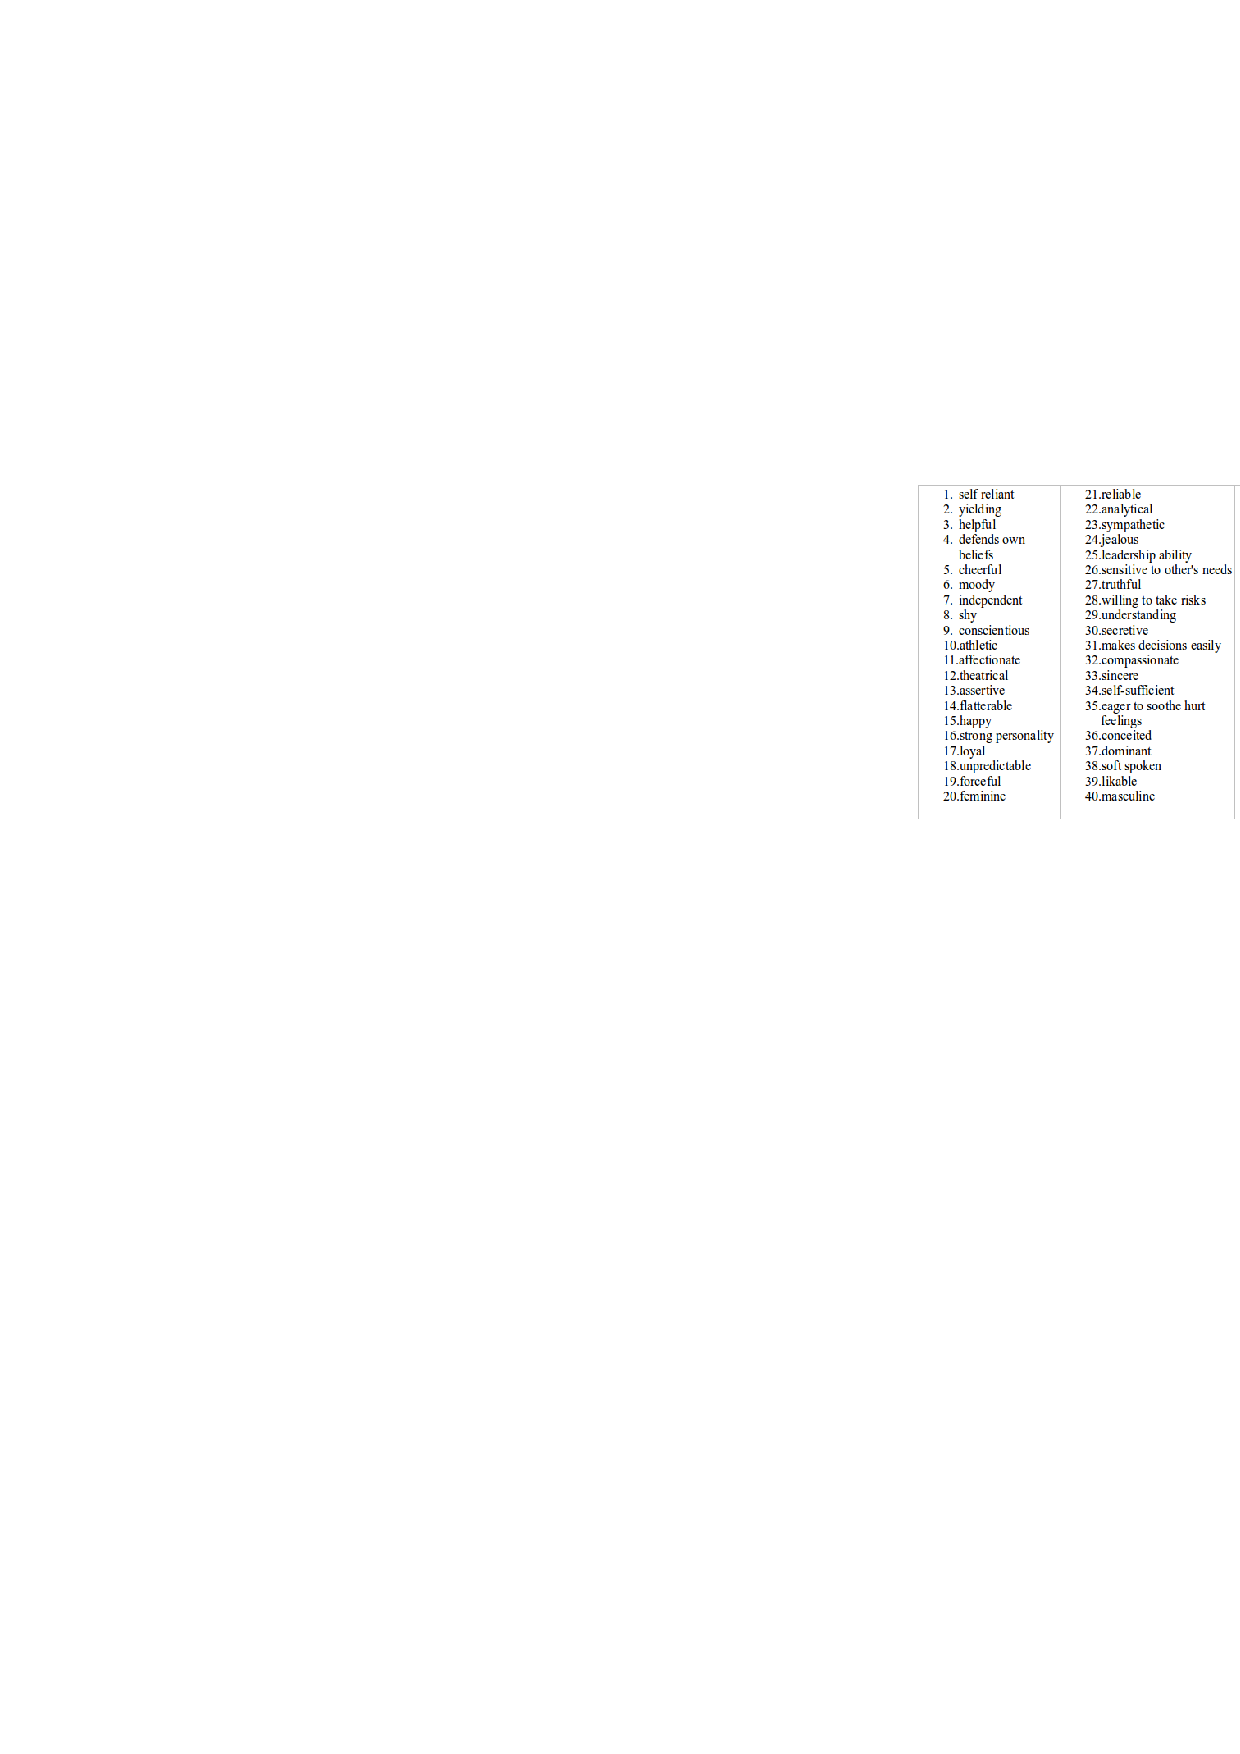
\includegraphics[width=4.5in]{bem}

\end{frame}

\begin{frame}[fragile]{Some of the data, and making a scree plot}

  {\footnotesize
\begin{knitrout}
\definecolor{shadecolor}{rgb}{0.969, 0.969, 0.969}\color{fgcolor}\begin{kframe}
\begin{alltt}
\hlstd{bem}\hlkwb{=}\hlkwd{read.table}\hlstd{(}\hlstr{"factor.txt"}\hlstd{,}\hlkwc{header}\hlstd{=T)}
\hlstd{bem[}\hlnum{1}\hlopt{:}\hlnum{10}\hlstd{,}\hlnum{2}\hlopt{:}\hlnum{9}\hlstd{]}
\end{alltt}
\begin{verbatim}
##    helpful reliant defbel yielding cheerful indpt athlet shy
## 1        7       7      5        5        7     7      7   1
## 2        5       6      6        6        2     3      3   3
## 3        7       6      4        4        5     5      2   3
## 4        6       6      7        4        6     6      3   4
## 5        6       6      7        4        7     7      7   2
## 6        5       6      7        4        6     6      2   4
## 7        6       4      6        6        6     3      1   3
## 8        7       6      7        5        6     7      5   2
## 9        7       6      6        4        4     5      2   2
## 10       7       4      7        4        7     5      2   1
\end{verbatim}
\begin{alltt}
\hlstd{bem.pc}\hlkwb{=}\hlkwd{princomp}\hlstd{(bem[,}\hlopt{-}\hlnum{1}\hlstd{],}\hlkwc{cor}\hlstd{=T)}
\end{alltt}
\end{kframe}
\end{knitrout}
}

\begin{knitrout}
\definecolor{shadecolor}{rgb}{0.969, 0.969, 0.969}\color{fgcolor}\begin{kframe}
\begin{alltt}
\hlkwd{plot}\hlstd{(bem.pc}\hlopt{$}\hlstd{sdev}\hlopt{^}\hlnum{2}\hlstd{,}\hlkwc{type}\hlstd{=}\hlstr{"b"}\hlstd{)}
\hlkwd{abline}\hlstd{(}\hlkwc{h}\hlstd{=}\hlnum{1}\hlstd{,}\hlkwc{lty}\hlstd{=}\hlstr{"dashed"}\hlstd{)}
\end{alltt}
\end{kframe}
\end{knitrout}

%$
\end{frame}

\begin{frame}[fragile]{The scree plot}
 
\begin{knitrout}
\definecolor{shadecolor}{rgb}{0.969, 0.969, 0.969}\color{fgcolor}
\includegraphics[width=\maxwidth]{figure/genoa-1} 

\end{knitrout}

  \begin{itemize}
  \item No obvious elbow.
  \item \emph{Lots} of eigenvalues bigger than 1.
  \end{itemize}

  
%  \includegraphics[height=\textheight]{bFactor-bem-scree}
\end{frame}

\begin{frame}[fragile]{Zoom in to search for elbow}
  
\begin{knitrout}
\definecolor{shadecolor}{rgb}{0.969, 0.969, 0.969}\color{fgcolor}\begin{kframe}
\begin{alltt}
\hlkwd{plot}\hlstd{(bem.pc}\hlopt{$}\hlstd{sdev}\hlopt{^}\hlnum{2}\hlstd{,}\hlkwc{type}\hlstd{=}\hlstr{"b"}\hlstd{,}\hlkwc{xlim}\hlstd{=}\hlkwd{c}\hlstd{(}\hlnum{0}\hlstd{,}\hlnum{10}\hlstd{))}
\hlkwd{abline}\hlstd{(}\hlkwc{h}\hlstd{=}\hlnum{1}\hlstd{,}\hlkwc{lty}\hlstd{=}\hlstr{"dashed"}\hlstd{)}
\end{alltt}
\end{kframe}
\includegraphics[width=\maxwidth]{figure/bem-scree-two-1} 

\end{knitrout}
  
\end{frame}

\begin{frame}[fragile]{but is 2 really good?}
  
  {\scriptsize
\begin{knitrout}
\definecolor{shadecolor}{rgb}{0.969, 0.969, 0.969}\color{fgcolor}\begin{kframe}
\begin{alltt}
\hlkwd{summary}\hlstd{(bem.pc)}
\end{alltt}
\begin{verbatim}
## Importance of components:
##                           Comp.1    Comp.2     Comp.3     Comp.4
## Standard deviation     2.7444993 2.2405789 1.55049106 1.43886350
## Proportion of Variance 0.1711881 0.1140953 0.05463688 0.04705291
## Cumulative Proportion  0.1711881 0.2852834 0.33992029 0.38697320
##                            Comp.5     Comp.6     Comp.7     Comp.8
## Standard deviation     1.30318840 1.18837867 1.15919129 1.07838912
## Proportion of Variance 0.03859773 0.03209645 0.03053919 0.02643007
## Cumulative Proportion  0.42557093 0.45766738 0.48820657 0.51463664
##                            Comp.9    Comp.10    Comp.11    Comp.12
## Standard deviation     1.07120568 1.04901318 1.03848656 1.00152287
## Proportion of Variance 0.02607913 0.02500974 0.02451033 0.02279655
## Cumulative Proportion  0.54071577 0.56572551 0.59023584 0.61303238
##                           Comp.13    Comp.14   Comp.15    Comp.16
## Standard deviation     0.97753974 0.95697572 0.9287543 0.92262649
## Proportion of Variance 0.02171782 0.02081369 0.0196042 0.01934636
## Cumulative Proportion  0.63475020 0.65556390 0.6751681 0.69451445
##                           Comp.17   Comp.18    Comp.19    Comp.20
## Standard deviation     0.90585705 0.8788668 0.86757525 0.84269120
## Proportion of Variance 0.01864948 0.0175547 0.01710652 0.01613928
## Cumulative Proportion  0.71316392 0.7307186 0.74782514 0.76396443
##                           Comp.21    Comp.22    Comp.23    Comp.24
## Standard deviation     0.83124925 0.80564654 0.78975423 0.78100835
## Proportion of Variance 0.01570398 0.01475151 0.01417527 0.01386305
## Cumulative Proportion  0.77966841 0.79441992 0.80859519 0.82245823
##                           Comp.25    Comp.26    Comp.27    Comp.28
## Standard deviation     0.77852606 0.74969868 0.74137885 0.72343693
## Proportion of Variance 0.01377506 0.01277382 0.01249188 0.01189457
## Cumulative Proportion  0.83623330 0.84900712 0.86149899 0.87339356
##                           Comp.29    Comp.30    Comp.31     Comp.32
## Standard deviation     0.71457305 0.70358645 0.69022738 0.654861232
## Proportion of Variance 0.01160488 0.01125077 0.01082759 0.009746437
## Cumulative Proportion  0.88499844 0.89624921 0.90707680 0.916823235
##                            Comp.33    Comp.34     Comp.35     Comp.36
## Standard deviation     0.640339974 0.63179848 0.616621295 0.602404917
## Proportion of Variance 0.009318984 0.00907203 0.008641405 0.008247538
## Cumulative Proportion  0.926142219 0.93521425 0.943855654 0.952103192
##                            Comp.37     Comp.38     Comp.39     Comp.40
## Standard deviation     0.570025368 0.560881809 0.538149460 0.530277613
## Proportion of Variance 0.007384748 0.007149736 0.006581928 0.006390781
## Cumulative Proportion  0.959487940 0.966637677 0.973219605 0.979610386
##                            Comp.41     Comp.42     Comp.43     Comp.44
## Standard deviation     0.512370708 0.505662309 0.480413465 0.384873772
## Proportion of Variance 0.005966449 0.005811236 0.005245389 0.003366541
## Cumulative Proportion  0.985576834 0.991388070 0.996633459 1.000000000
\end{verbatim}
\end{kframe}
\end{knitrout}
}

\end{frame}

\begin{frame}[fragile]{Comments}

  \begin{itemize}
\item Want overall fraction of variance explained (``cumulative
  proportion'') to be reasonably high.
\item 2 factors, 28.5\%. Terrible!
\item Even 56\% (10 factors) not that good!
\item Have to live with that.
\end{itemize}

\end{frame}

\begin{frame}[fragile]{Biplot version 1}

\begin{knitrout}
\definecolor{shadecolor}{rgb}{0.969, 0.969, 0.969}\color{fgcolor}\begin{kframe}
\begin{alltt}
\hlkwd{biplot}\hlstd{(bem.pc)}
\end{alltt}
\end{kframe}
\includegraphics[width=\maxwidth]{figure/bem-biplot-1} 

\end{knitrout}
%  \includegraphics[height=0.8\textheight]{bFactor-bem-biplot}
  
\end{frame}

\begin{frame}{Biplot version 2 (less busy)}

Shrink individuals (1st thing in \texttt{cex}), variables (2nd):
\begin{knitrout}
\definecolor{shadecolor}{rgb}{0.969, 0.969, 0.969}\color{fgcolor}\begin{kframe}
\begin{alltt}
\hlkwd{biplot}\hlstd{(bem.pc,}\hlkwc{cex}\hlstd{=}\hlkwd{c}\hlstd{(}\hlnum{0.25}\hlstd{,}\hlnum{0.5}\hlstd{))}
\end{alltt}
\end{kframe}
\includegraphics[width=\maxwidth]{figure/bem-biplot-two-1} 

\end{knitrout}

%  \includegraphics[height=\textheight]{bFactor-bem-biplot-two}
  
\end{frame}

\begin{frame}[fragile]{Comments}
  
  \begin{itemize}
  \item Ignore individuals for now.
  \item Most variables point to 10 o'clock or 7 o'clock.
  \item Suggests factor analysis with rotation will get interpretable
    factors (rotate to 6 o'clock and 9 o'clock, for example).
  \item Try for 2-factor solution (rough interpretation, will be bad):
\begin{knitrout}
\definecolor{shadecolor}{rgb}{0.969, 0.969, 0.969}\color{fgcolor}\begin{kframe}
\begin{alltt}
\hlstd{bem.2}\hlkwb{=}\hlkwd{factanal}\hlstd{(bem[,}\hlopt{-}\hlnum{1}\hlstd{],}\hlkwc{factors}\hlstd{=}\hlnum{2}\hlstd{)}
\end{alltt}
\end{kframe}
\end{knitrout}
\item Show output in pieces (just print \texttt{bem.2} to see all of it).
  \end{itemize}
  
\end{frame}

\begin{frame}[fragile]{Uniquenesses}
  
{\scriptsize  
\begin{knitrout}
\definecolor{shadecolor}{rgb}{0.969, 0.969, 0.969}\color{fgcolor}\begin{kframe}
\begin{alltt}
\hlstd{bem.2}\hlopt{$}\hlstd{uniquenesses}
\end{alltt}
\begin{verbatim}
##   helpful   reliant    defbel  yielding  cheerful     indpt    athlet 
## 0.7598223 0.7808058 0.7748448 0.8688473 0.8394916 0.7282742 0.9229702 
##       shy    assert   strpers  forceful    affect   flatter     loyal 
## 0.8239496 0.6329347 0.5679398 0.5631857 0.6616625 0.9409500 0.8035264 
##    analyt  feminine  sympathy     moody  sensitiv  undstand   compass 
## 0.8968744 0.8829927 0.7231450 0.9730607 0.8018851 0.6194392 0.5937073 
##  leaderab    soothe      risk    decide  selfsuff  conscien  dominant 
## 0.4091894 0.6596103 0.7789761 0.6938578 0.7210246 0.7974820 0.4942909 
##  masculin     stand     happy  softspok      warm  truthful    tender 
## 0.8453368 0.6024001 0.8008966 0.8339058 0.4764762 0.8889983 0.4928919 
##  gullible   leadact  childlik   individ  foullang   lovchil   compete 
## 0.9583435 0.4166153 0.9800360 0.7941998 0.9821662 0.8924392 0.7942910 
##  ambitiou    gentle 
## 0.8101599 0.5064551
\end{verbatim}
\end{kframe}
\end{knitrout}
}

\begin{itemize}
\item Mostly high or very high (bad).
\item Some smaller, eg.:
  Leadership ability (0.409),
  Acts like leader (0.417),
  Warm (0.476),
  Tender (0.493).
\item Smaller uniquenesses captured by one of our two factors.
\end{itemize}
  
\end{frame}

\begin{frame}[fragile]{Factor 1}

 Just \texttt{bem.2\$loadings} to see both factors. Or only factor 1:

 {\scriptsize
\begin{knitrout}
\definecolor{shadecolor}{rgb}{0.969, 0.969, 0.969}\color{fgcolor}\begin{kframe}
\begin{alltt}
\hlstd{bem.2}\hlopt{$}\hlstd{loadings[,}\hlnum{1}\hlstd{]}
\end{alltt}
\begin{verbatim}
##      helpful      reliant       defbel     yielding     cheerful 
##  0.313746590  0.453290387  0.433657422 -0.130996520  0.152371766 
##        indpt       athlet          shy       assert      strpers 
##  0.521240328  0.267078824 -0.414457941  0.604958754  0.656985468 
##     forceful       affect      flatter        loyal       analyt 
##  0.648719028  0.177891120  0.096422637  0.151212661  0.294955876 
##     feminine     sympathy        moody     sensitiv     undstand 
##  0.113201861  0.023014564 -0.023305420  0.134769700  0.091112993 
##      compass     leaderab       soothe         risk       decide 
##  0.113506433  0.765492393  0.060617547  0.441617628  0.541679637 
##     selfsuff     conscien     dominant     masculin        stand 
##  0.510996369  0.327762957  0.667649029  0.275876974  0.606686424 
##        happy     softspok         warm     truthful       tender 
##  0.118930114 -0.230328343  0.079569783  0.109122076  0.051138067 
##     gullible      leadact     childlik      individ     foullang 
## -0.152850183  0.762712949 -0.101438396  0.444806432 -0.004928512 
##      lovchil      compete     ambitiou       gentle 
## -0.027057152  0.450418755  0.413649844 -0.018732236
\end{verbatim}
\end{kframe}
\end{knitrout}
}

%$


  
\end{frame}

\begin{frame}[fragile]{Or pick out the big ones}

Arbitrarily defining $>0.4$ or $<-0.4$ as ``big'':



{\small
\begin{knitrout}
\definecolor{shadecolor}{rgb}{0.969, 0.969, 0.969}\color{fgcolor}\begin{kframe}
\begin{alltt}
\hlstd{big}\hlkwb{=}\hlkwd{abs}\hlstd{(bem.2}\hlopt{$}\hlstd{loadings[,}\hlnum{1}\hlstd{])}\hlopt{>}\hlnum{0.4}
\hlstd{bem.2}\hlopt{$}\hlstd{loadings[big,}\hlnum{1}\hlstd{]}
\end{alltt}
\begin{verbatim}
##    reliant     defbel      indpt        shy     assert 
##  0.4532904  0.4336574  0.5212403 -0.4144579  0.6049588 
##    strpers   forceful   leaderab       risk     decide 
##  0.6569855  0.6487190  0.7654924  0.4416176  0.5416796 
##   selfsuff   dominant      stand    leadact    individ 
##  0.5109964  0.6676490  0.6066864  0.7627129  0.4448064 
##    compete   ambitiou 
##  0.4504188  0.4136498
\end{verbatim}
\end{kframe}
\end{knitrout}
}

 ``Traditional masculine'' traits, including
  ``not-shy'' (negative loading).

\end{frame}

\begin{frame}[fragile]{Factor 2, the big ones}
  
{\small  
\begin{knitrout}
\definecolor{shadecolor}{rgb}{0.969, 0.969, 0.969}\color{fgcolor}\begin{kframe}
\begin{alltt}
\hlstd{big}\hlkwb{=}\hlkwd{abs}\hlstd{(bem.2}\hlopt{$}\hlstd{loadings[,}\hlnum{2}\hlstd{])}\hlopt{>}\hlnum{0.4}
\hlstd{bem.2}\hlopt{$}\hlstd{loadings[big,}\hlnum{2}\hlstd{]}
\end{alltt}
\begin{verbatim}
##    affect     loyal  sympathy  sensitiv  undstand   compass 
## 0.5537994 0.4166622 0.5256654 0.4242037 0.6101294 0.6272223 
##    soothe     happy      warm    tender    gentle 
## 0.5802714 0.4300698 0.7191610 0.7102763 0.7022768
\end{verbatim}
\end{kframe}
\end{knitrout}
}

``Traditional feminine'' traits.

\end{frame}

\begin{frame}[fragile]{Plotting the two factors}
  
A bi-plot, this time with the variables reduced in size. Looking for
unusual individuals.

Have to run \texttt{factanal} again to get factor scores for plotting.

\begin{knitrout}
\definecolor{shadecolor}{rgb}{0.969, 0.969, 0.969}\color{fgcolor}\begin{kframe}
\begin{alltt}
\hlstd{bem.2a}\hlkwb{=}\hlkwd{factanal}\hlstd{(bem[,}\hlopt{-}\hlnum{1}\hlstd{],}\hlkwc{factors}\hlstd{=}\hlnum{2}\hlstd{,}\hlkwc{scores}\hlstd{=}\hlstr{"r"}\hlstd{)}
\hlkwd{biplot}\hlstd{(bem.2a}\hlopt{$}\hlstd{scores,bem.2a}\hlopt{$}\hlstd{loadings,}\hlkwc{cex}\hlstd{=}\hlkwd{c}\hlstd{(}\hlnum{0.75}\hlstd{,}\hlnum{0.5}\hlstd{))}
\end{alltt}
\end{kframe}
\end{knitrout}

Numbers on plot are row numbers of \texttt{bem}
data frame.
  
\end{frame}

\begin{frame}[fragile]{The biplot}
  
%\includegraphics[height=\textheight]{bFactor-biplot-two-again} 
  
\begin{knitrout}
\definecolor{shadecolor}{rgb}{0.969, 0.969, 0.969}\color{fgcolor}
\includegraphics[width=\maxwidth]{figure/biplot-two-ag-1} 

\end{knitrout}
  
  
\end{frame}

\begin{frame}[fragile]{Comments}
  
  \begin{itemize}
  \item Variables mostly up (``feminine'') and right (``masculine''),
    accomplished by rotation.
  \item Some unusual individuals: 311, 214 (low on factor 2), 366
    (high on factor 2),
    359, 258
    (low on factor 1), 230 (high on factor 1).
  \item Pick out variables going with each factor and list these rows
    and columns of \texttt{bem} for each factor:
\begin{knitrout}
\definecolor{shadecolor}{rgb}{0.969, 0.969, 0.969}\color{fgcolor}\begin{kframe}
\begin{alltt}
\hlstd{big1}\hlkwb{=}\hlkwd{abs}\hlstd{(bem.2}\hlopt{$}\hlstd{loadings[,}\hlnum{1}\hlstd{])}\hlopt{>}\hlnum{0.4}
\hlstd{big1}\hlkwb{=}\hlkwd{c}\hlstd{(}\hlnum{FALSE}\hlstd{,big1)}
\hlstd{big2}\hlkwb{=}\hlkwd{abs}\hlstd{(bem.2}\hlopt{$}\hlstd{loadings[,}\hlnum{2}\hlstd{])}\hlopt{>}\hlnum{0.4}
\hlstd{big2}\hlkwb{=}\hlkwd{c}\hlstd{(}\hlnum{FALSE}\hlstd{,big2)}
\end{alltt}
\end{kframe}
\end{knitrout}
  \end{itemize}


  
\end{frame}

\begin{frame}[fragile]{Factor 1}

  {\small
\begin{knitrout}
\definecolor{shadecolor}{rgb}{0.969, 0.969, 0.969}\color{fgcolor}\begin{kframe}
\begin{alltt}
\hlstd{bem[}\hlkwd{c}\hlstd{(}\hlnum{359}\hlstd{,}\hlnum{258}\hlstd{,}\hlnum{230}\hlstd{),big1]}
\end{alltt}
\begin{verbatim}
##     reliant defbel indpt shy assert strpers forceful
## 359       1      1     1   5      1       3        1
## 258       4      1     7   7      3       1        1
## 230       7      7     7   2      7       7        7
##     leaderab risk decide selfsuff dominant stand
## 359        1    7      2        1        1     6
## 258        1    5      1        4        1     1
## 230        7    7      7        7        7     7
##     leadact individ compete ambitiou
## 359       1       3       1        4
## 258       1       3       2        2
## 230       7       7       6        7
\end{verbatim}
\end{kframe}
\end{knitrout}
}

These are extreme scores on the things that go with factor 1 (first
two small, last one big).

\end{frame}

\begin{frame}[fragile]{Factor 2}
 
  {\small
\begin{knitrout}
\definecolor{shadecolor}{rgb}{0.969, 0.969, 0.969}\color{fgcolor}\begin{kframe}
\begin{alltt}
\hlstd{bem[}\hlkwd{c}\hlstd{(}\hlnum{311}\hlstd{,}\hlnum{214}\hlstd{,}\hlnum{366}\hlstd{),big2]}
\end{alltt}
\begin{verbatim}
##     affect loyal sympathy sensitiv undstand compass
## 311      5     4        4        4        3       4
## 214      1     7        4        7        5       5
## 366      7     7        7        7        7       6
##     soothe happy warm tender gentle
## 311      4     3    3      4      3
## 214      3     4    1      3      2
## 366      7     7    7      7      7
\end{verbatim}
\end{kframe}
\end{knitrout}
}

These are extreme scores on the things that go with factor 2 (first
two small, last one big).
  
\end{frame}
  

\begin{frame}[fragile]{Is 2 factors enough?}
  
  Suspect not:
  
\begin{knitrout}
\definecolor{shadecolor}{rgb}{0.969, 0.969, 0.969}\color{fgcolor}\begin{kframe}
\begin{alltt}
\hlstd{bem.2}\hlopt{$}\hlstd{PVAL}
\end{alltt}
\begin{verbatim}
##     objective 
## 1.458183e-150
\end{verbatim}
\end{kframe}
\end{knitrout}

2 factors resoundingly rejected. Need more. Have to go all the way to
15 factors to not reject:

\begin{knitrout}
\definecolor{shadecolor}{rgb}{0.969, 0.969, 0.969}\color{fgcolor}\begin{kframe}
\begin{alltt}
\hlstd{bem.15}\hlkwb{=}\hlkwd{factanal}\hlstd{(bem[,}\hlopt{-}\hlnum{1}\hlstd{],}\hlkwc{factors}\hlstd{=}\hlnum{15}\hlstd{)}
\hlstd{bem.15}\hlopt{$}\hlstd{PVAL}
\end{alltt}
\begin{verbatim}
## objective 
##  0.132617
\end{verbatim}
\end{kframe}
\end{knitrout}

Even then, only just over 50\% of variability explained.

Let's have a look at the important things in those 15 factors.

\end{frame}

\begin{frame}[fragile]{A loop}
  
  To save myself some effort:
  
\begin{knitrout}
\definecolor{shadecolor}{rgb}{0.969, 0.969, 0.969}\color{fgcolor}\begin{kframe}
\begin{alltt}
\hlstd{mylist}\hlkwb{=}\hlkwd{list}\hlstd{(}\hlkwd{list}\hlstd{())}
\hlkwa{for} \hlstd{(i} \hlkwa{in} \hlnum{1}\hlopt{:}\hlnum{15}\hlstd{)}
\hlstd{\{}
  \hlstd{v}\hlkwb{=}\hlkwd{sort}\hlstd{(bem.15}\hlopt{$}\hlstd{loadings[,i])}
  \hlstd{mylist[[i]]}\hlkwb{=}\hlkwd{round}\hlstd{(v,}\hlnum{2}\hlstd{)}
\hlstd{\}}
\end{alltt}
\end{kframe}
\end{knitrout}


%$
and then look at corresponding elements of \texttt{mylist}.
  
\end{frame}

\begin{frame}[fragile]{Factor 1}

  {\footnotesize
\begin{knitrout}
\definecolor{shadecolor}{rgb}{0.969, 0.969, 0.969}\color{fgcolor}\begin{kframe}
\begin{alltt}
\hlstd{mylist[[}\hlnum{1}\hlstd{]]}
\end{alltt}
\begin{verbatim}
## childlik masculin dominant      shy    indpt  compete 
##    -0.11    -0.10    -0.08    -0.05    -0.04    -0.03 
##  individ  leadact forceful   athlet  strpers foullang 
##    -0.02    -0.02    -0.01     0.00     0.03     0.03 
##    moody selfsuff ambitiou   decide    happy  flatter 
##     0.04     0.04     0.05     0.06     0.06     0.06 
##   assert softspok leaderab gullible   analyt     risk 
##     0.07     0.08     0.09     0.10     0.10     0.11 
##    stand cheerful  reliant feminine  lovchil    loyal 
##     0.11     0.13     0.13     0.13     0.14     0.17 
## truthful   defbel   affect yielding conscien  helpful 
##     0.18     0.18     0.20     0.21     0.23     0.25 
##   tender   gentle     warm   soothe sensitiv sympathy 
##     0.28     0.28     0.35     0.60     0.64     0.66 
## undstand  compass 
##     0.68     0.81
\end{verbatim}
\end{kframe}
\end{knitrout}
}

Soothing, sensitive, sympathetic, understanding, compassionate:
Thoughtful of others.
  
\end{frame}

\begin{frame}[fragile]{Factor 2}
  
  {\footnotesize
\begin{knitrout}
\definecolor{shadecolor}{rgb}{0.969, 0.969, 0.969}\color{fgcolor}\begin{kframe}
\begin{alltt}
\hlstd{mylist[[}\hlnum{2}\hlstd{]]}
\end{alltt}
\begin{verbatim}
## softspok      shy yielding  lovchil foullang   gentle 
##    -0.31    -0.29    -0.17    -0.06    -0.05    -0.02 
##     warm sympathy gullible    happy   tender   soothe 
##    -0.02    -0.01     0.00     0.00     0.00     0.01 
##  helpful feminine truthful undstand sensitiv childlik 
##     0.02     0.02     0.02     0.02     0.04     0.05 
##    moody cheerful  compass conscien   athlet    loyal 
##     0.05     0.05     0.08     0.08     0.08     0.10 
##  flatter ambitiou  reliant   affect  individ  compete 
##     0.11     0.13     0.15     0.15     0.19     0.19 
## masculin selfsuff     risk    indpt   defbel   decide 
##     0.20     0.21     0.21     0.22     0.23     0.24 
##   analyt  leadact    stand leaderab dominant   assert 
##     0.26     0.35     0.37     0.39     0.50     0.70 
## forceful  strpers 
##     0.72     0.76
\end{verbatim}
\end{kframe}
\end{knitrout}
}

Dominant, assertive, forceful, strong personality: Getting ahead.

\end{frame}

\begin{frame}[fragile]{Factor 3}
  
  {\small
\begin{knitrout}
\definecolor{shadecolor}{rgb}{0.969, 0.969, 0.969}\color{fgcolor}\begin{kframe}
\begin{alltt}
\hlstd{mylist[[}\hlnum{3}\hlstd{]]}
\end{alltt}
\begin{verbatim}
## gullible childlik    moody  flatter      shy   soothe 
##    -0.34    -0.14    -0.10    -0.07    -0.07    -0.07 
##  lovchil yielding foullang   gentle     warm sympathy 
##    -0.04    -0.04    -0.03    -0.03     0.00     0.00 
##   affect  compete   tender masculin    loyal    happy 
##     0.03     0.05     0.05     0.06     0.07     0.07 
## truthful   athlet sensitiv softspok  compass feminine 
##     0.07     0.08     0.09     0.10     0.10     0.10 
## forceful     risk undstand   analyt cheerful  strpers 
##     0.11     0.12     0.14     0.15     0.15     0.15 
## ambitiou   assert dominant  leadact    stand   defbel 
##     0.17     0.18     0.18     0.21     0.21     0.28 
## leaderab conscien   decide  individ  helpful    indpt 
##     0.29     0.33     0.33     0.33     0.39     0.62 
## selfsuff  reliant 
##     0.65     0.67
\end{verbatim}
\end{kframe}
\end{knitrout}
}

Independent, self-sufficient, self-reliant: Going it alone.

\end{frame}
\begin{frame}[fragile]{Factor 4}
  
  {\small
\begin{knitrout}
\definecolor{shadecolor}{rgb}{0.969, 0.969, 0.969}\color{fgcolor}\begin{kframe}
\begin{alltt}
\hlstd{mylist[[}\hlnum{4}\hlstd{]]}
\end{alltt}
\begin{verbatim}
## dominant masculin    moody forceful  reliant  leadact 
##    -0.19    -0.14    -0.10    -0.09    -0.07    -0.04 
##  strpers    indpt   athlet  individ   defbel   assert 
##    -0.03    -0.01     0.01     0.01     0.04     0.04 
## sensitiv  compete leaderab childlik   decide      shy 
##     0.05     0.05     0.05     0.05     0.06     0.07 
## selfsuff    stand  flatter foullang   analyt ambitiou 
##     0.07     0.07     0.08     0.10     0.10     0.10 
## sympathy feminine truthful cheerful     risk conscien 
##     0.10     0.12     0.12     0.14     0.14     0.15 
##  helpful yielding  compass gullible   soothe    loyal 
##     0.17     0.18     0.19     0.19     0.20     0.21 
##    happy undstand  lovchil softspok   affect     warm 
##     0.24     0.24     0.28     0.39     0.45     0.60 
##   tender   gentle 
##     0.69     0.70
\end{verbatim}
\end{kframe}
\end{knitrout}
}

Affectionate, warm, gentle, tender: Caring for others.

\end{frame}
\begin{frame}[fragile]{Factor 5}
  
  {\footnotesize
\begin{knitrout}
\definecolor{shadecolor}{rgb}{0.969, 0.969, 0.969}\color{fgcolor}\begin{kframe}
\begin{alltt}
\hlstd{mylist[[}\hlnum{5}\hlstd{]]}
\end{alltt}
\begin{verbatim}
##      shy  compass truthful softspok childlik undstand 
##    -0.10    -0.02    -0.02    -0.01    -0.01    -0.01 
## sympathy    loyal feminine   affect    moody sensitiv 
##     0.00     0.00     0.01     0.01     0.02     0.03 
##   defbel cheerful     warm  reliant forceful yielding 
##     0.03     0.03     0.03     0.05     0.05     0.05 
##  lovchil   soothe   assert  helpful    happy  flatter 
##     0.07     0.07     0.09     0.09     0.09     0.10 
##   tender masculin gullible    indpt conscien    stand 
##     0.10     0.11     0.12     0.13     0.13     0.13 
##   analyt   gentle foullang selfsuff  strpers  leadact 
##     0.13     0.15     0.17     0.18     0.19     0.19 
## dominant   decide leaderab   athlet  individ     risk 
##     0.21     0.24     0.27     0.28     0.34     0.35 
## ambitiou  compete 
##     0.67     0.70
\end{verbatim}
\end{kframe}
\end{knitrout}
}

Ambitious, competitive (with a bit of risk-taking and individualism):
Being the best.

\end{frame}
\begin{frame}[fragile]{Factor 6}
  
  {\footnotesize
\begin{knitrout}
\definecolor{shadecolor}{rgb}{0.969, 0.969, 0.969}\color{fgcolor}\begin{kframe}
\begin{alltt}
\hlstd{mylist[[}\hlnum{6}\hlstd{]]}
\end{alltt}
\begin{verbatim}
##      shy childlik softspok   gentle foullang yielding 
##    -0.19    -0.05    -0.05    -0.05    -0.05    -0.04 
##    moody sympathy   tender    happy  lovchil  flatter 
##    -0.03    -0.02    -0.01    -0.01    -0.01     0.00 
##   analyt    loyal  compass undstand truthful sensitiv 
##     0.01     0.01     0.01     0.01     0.01     0.01 
##   soothe gullible cheerful selfsuff   affect  individ 
##     0.02     0.02     0.03     0.04     0.05     0.05 
## feminine   assert     warm ambitiou conscien  strpers 
##     0.05     0.05     0.07     0.08     0.09     0.10 
##  reliant    indpt    stand   defbel  helpful   athlet 
##     0.11     0.11     0.12     0.13     0.15     0.15 
##  compete   decide masculin     risk forceful dominant 
##     0.16     0.16     0.17     0.18     0.20     0.34 
## leaderab  leadact 
##     0.61     0.87
\end{verbatim}
\end{kframe}
\end{knitrout}
}

Acts like a leader, leadership ability (with a bit of Dominant):
Taking charge.

\end{frame}
\begin{frame}[fragile]{Factor 7}
  
  {\small
\begin{knitrout}
\definecolor{shadecolor}{rgb}{0.969, 0.969, 0.969}\color{fgcolor}\begin{kframe}
\begin{alltt}
\hlstd{mylist[[}\hlnum{7}\hlstd{]]}
\end{alltt}
\begin{verbatim}
##    moody masculin      shy dominant   analyt childlik 
##    -0.52    -0.16    -0.13    -0.13    -0.10    -0.10 
## sensitiv   defbel forceful sympathy ambitiou gullible 
##    -0.04    -0.03    -0.03    -0.02    -0.02    -0.02 
##   assert    stand leaderab conscien     risk  compete 
##     0.00     0.00     0.01     0.01     0.02     0.03 
## softspok   affect undstand    indpt  individ selfsuff 
##     0.03     0.04     0.04     0.05     0.05     0.05 
## feminine  flatter  leadact  compass foullang   tender 
##     0.07     0.07     0.08     0.08     0.09     0.09 
##  helpful   decide    loyal truthful  strpers   soothe 
##     0.10     0.10     0.10     0.10     0.12     0.13 
##  lovchil yielding  reliant   gentle     warm   athlet 
##     0.14     0.15     0.16     0.17     0.21     0.22 
## cheerful    happy 
##     0.67     0.67
\end{verbatim}
\end{kframe}
\end{knitrout}
}

Happy, cheerful, not-moody: Optimistic.

\end{frame}
\begin{frame}[fragile]{Factor 8}
  
  {\small
\begin{knitrout}
\definecolor{shadecolor}{rgb}{0.969, 0.969, 0.969}\color{fgcolor}\begin{kframe}
\begin{alltt}
\hlstd{mylist[[}\hlnum{8}\hlstd{]]}
\end{alltt}
\begin{verbatim}
## softspok      shy selfsuff conscien masculin   decide 
##    -0.25    -0.18    -0.13    -0.12    -0.12    -0.11 
## foullang   analyt    indpt  compass   gentle sensitiv 
##    -0.08    -0.06    -0.05    -0.04    -0.03    -0.02 
## undstand     risk dominant ambitiou forceful  reliant 
##    -0.01    -0.01     0.00     0.00     0.01     0.01 
##    stand  individ  leadact leaderab gullible truthful 
##     0.01     0.02     0.02     0.02     0.04     0.05 
## childlik yielding  lovchil   assert sympathy    happy 
##     0.05     0.07     0.09     0.10     0.11     0.11 
##   soothe   defbel feminine    moody   athlet cheerful 
##     0.13     0.14     0.14     0.15     0.15     0.15 
##  helpful    loyal  compete  strpers   tender     warm 
##     0.15     0.17     0.18     0.18     0.19     0.22 
##  flatter   affect 
##     0.52     0.63
\end{verbatim}
\end{kframe}
\end{knitrout}
}

Affectionate, flattering: Making others feel good.

\end{frame}
\begin{frame}[fragile]{Factor 9}
  
  {\small
\begin{knitrout}
\definecolor{shadecolor}{rgb}{0.969, 0.969, 0.969}\color{fgcolor}\begin{kframe}
\begin{alltt}
\hlstd{mylist[[}\hlnum{9}\hlstd{]]}
\end{alltt}
\begin{verbatim}
##      shy gullible yielding undstand   athlet ambitiou 
##    -0.17    -0.11    -0.03    -0.03    -0.01     0.00 
##  flatter   gentle  compete childlik softspok sympathy 
##     0.00     0.01     0.01     0.01     0.02     0.02 
##   tender masculin  compass  lovchil  reliant feminine 
##     0.02     0.02     0.02     0.02     0.02     0.02 
## cheerful    happy    loyal    moody selfsuff    indpt 
##     0.03     0.03     0.04     0.05     0.05     0.06 
## dominant truthful   soothe  helpful   affect forceful 
##     0.07     0.07     0.07     0.07     0.07     0.08 
##  strpers sensitiv foullang  leadact leaderab     warm 
##     0.08     0.10     0.10     0.10     0.10     0.10 
##   analyt conscien   assert   decide     risk  individ 
##     0.11     0.12     0.12     0.17     0.19     0.24 
##   defbel    stand 
##     0.34     0.86
\end{verbatim}
\end{kframe}
\end{knitrout}
}

Taking a stand.

\end{frame}
\begin{frame}[fragile]{Factor 10}
  
  {\small
\begin{knitrout}
\definecolor{shadecolor}{rgb}{0.969, 0.969, 0.969}\color{fgcolor}\begin{kframe}
\begin{alltt}
\hlstd{mylist[[}\hlnum{10}\hlstd{]]}
\end{alltt}
\begin{verbatim}
## masculin  lovchil   athlet    indpt  compete  helpful 
##    -0.26    -0.09    -0.09    -0.08    -0.07    -0.05 
##      shy   assert childlik  strpers    loyal   defbel 
##    -0.03    -0.03    -0.03    -0.02    -0.02    -0.02 
##    moody leaderab gullible truthful   analyt forceful 
##     0.00     0.00     0.00     0.01     0.01     0.01 
## sensitiv    stand     risk ambitiou  leadact  compass 
##     0.02     0.02     0.02     0.02     0.03     0.03 
##   soothe dominant undstand foullang   tender  reliant 
##     0.03     0.05     0.05     0.06     0.06     0.07 
## cheerful   affect    happy     warm sympathy  individ 
##     0.07     0.08     0.08     0.08     0.09     0.09 
##   decide  flatter   gentle yielding selfsuff conscien 
##     0.11     0.11     0.14     0.18     0.20     0.23 
## softspok feminine 
##     0.25     0.81
\end{verbatim}
\end{kframe}
\end{knitrout}
}

Feminine. (A little bit of not-masculine!)

\end{frame}
\begin{frame}[fragile]{Factor 11}
  
  {\small
\begin{knitrout}
\definecolor{shadecolor}{rgb}{0.969, 0.969, 0.969}\color{fgcolor}\begin{kframe}
\begin{alltt}
\hlstd{mylist[[}\hlnum{11}\hlstd{]]}
\end{alltt}
\begin{verbatim}
##   athlet dominant  compete childlik yielding leaderab 
##    -0.06    -0.04    -0.03    -0.02    -0.01    -0.01 
## feminine softspok selfsuff     risk  reliant    indpt 
##    -0.01     0.00     0.00     0.00     0.01     0.01 
##     warm forceful undstand  strpers ambitiou    stand 
##     0.01     0.02     0.02     0.02     0.02     0.03 
##  leadact    moody sympathy sensitiv  compass foullang 
##     0.03     0.03     0.03     0.04     0.04     0.05 
##  individ   assert   defbel   gentle  flatter    happy 
##     0.05     0.05     0.05     0.05     0.05     0.06 
##   soothe masculin      shy   decide conscien cheerful 
##     0.06     0.06     0.06     0.06     0.08     0.09 
## gullible  lovchil   tender   analyt  helpful truthful 
##     0.10     0.10     0.10     0.10     0.12     0.16 
##   affect    loyal 
##     0.19     0.92
\end{verbatim}
\end{kframe}
\end{knitrout}
}

Loyal.

\end{frame}
\begin{frame}[fragile]{Factor 12}
  
  {\footnotesize
\begin{knitrout}
\definecolor{shadecolor}{rgb}{0.969, 0.969, 0.969}\color{fgcolor}\begin{kframe}
\begin{alltt}
\hlstd{mylist[[}\hlnum{12}\hlstd{]]}
\end{alltt}
\begin{verbatim}
## selfsuff conscien   decide leaderab yielding   soothe 
##    -0.28    -0.28    -0.17    -0.13    -0.12    -0.10 
## undstand ambitiou  leadact    indpt truthful sympathy 
##    -0.09    -0.08    -0.08    -0.07    -0.06    -0.06 
##    stand   assert  helpful foullang    loyal  lovchil 
##    -0.06    -0.05    -0.05    -0.03    -0.03    -0.02 
## feminine sensitiv    happy   analyt  compete softspok 
##    -0.02    -0.02    -0.01    -0.01    -0.01    -0.01 
##   gentle cheerful   tender  reliant  strpers  flatter 
##    -0.01     0.02     0.02     0.03     0.03     0.05 
##   affect forceful     warm  individ   athlet   defbel 
##     0.06     0.06     0.07     0.09     0.10     0.11 
##     risk gullible  compass dominant masculin      shy 
##     0.11     0.13     0.14     0.15     0.15     0.20 
##    moody childlik 
##     0.26     0.61
\end{verbatim}
\end{kframe}
\end{knitrout}
}

Childlike. (With a bit of moody, shy, not-self-sufficient, not-conscientious.)

\end{frame}
\begin{frame}[fragile]{Factor 13}
  
  {\small
\begin{knitrout}
\definecolor{shadecolor}{rgb}{0.969, 0.969, 0.969}\color{fgcolor}\begin{kframe}
\begin{alltt}
\hlstd{mylist[[}\hlnum{13}\hlstd{]]}
\end{alltt}
\begin{verbatim}
## gullible      shy yielding   assert  lovchil cheerful 
##    -0.28    -0.17    -0.14    -0.13    -0.11    -0.10 
##   decide     risk childlik  reliant foullang    moody 
##    -0.08    -0.08    -0.06    -0.05    -0.05    -0.05 
##  leadact ambitiou   soothe selfsuff  compete  flatter 
##    -0.04    -0.03    -0.03    -0.02     0.00     0.01 
## feminine softspok masculin sympathy  strpers sensitiv 
##     0.02     0.02     0.02     0.03     0.04     0.04 
##   gentle   tender   affect forceful undstand leaderab 
##     0.05     0.05     0.05     0.05     0.06     0.07 
## conscien    indpt  compass  individ  helpful   athlet 
##     0.08     0.08     0.08     0.08     0.10     0.10 
##    stand dominant   analyt   defbel    loyal     warm 
##     0.10     0.10     0.11     0.11     0.16     0.19 
##    happy truthful 
##     0.26     0.57
\end{verbatim}
\end{kframe}
\end{knitrout}
}

Truthful. (With a bit of happy and not-gullible.)

\end{frame}
\begin{frame}[fragile]{Factor 14}
  
  {\small
\begin{knitrout}
\definecolor{shadecolor}{rgb}{0.969, 0.969, 0.969}\color{fgcolor}\begin{kframe}
\begin{alltt}
\hlstd{mylist[[}\hlnum{14}\hlstd{]]}
\end{alltt}
\begin{verbatim}
## softspok  strpers foullang  individ   analyt  helpful 
##    -0.19    -0.15    -0.09    -0.09    -0.09    -0.08 
## cheerful conscien  flatter leaderab  reliant   gentle 
##    -0.07    -0.06    -0.06    -0.05    -0.05    -0.04 
## childlik gullible truthful undstand sensitiv   soothe 
##    -0.04    -0.03    -0.03    -0.03    -0.02    -0.01 
## sympathy   tender yielding    moody ambitiou   athlet 
##    -0.01     0.00     0.01     0.01     0.02     0.02 
##    loyal   assert   defbel feminine      shy    stand 
##     0.02     0.03     0.05     0.06     0.06     0.07 
##  lovchil   affect    indpt     warm  compete  leadact 
##     0.07     0.08     0.08     0.08     0.09     0.10 
## masculin  compass    happy dominant     risk forceful 
##     0.11     0.12     0.13     0.15     0.16     0.19 
## selfsuff   decide 
##     0.24     0.44
\end{verbatim}
\end{kframe}
\end{knitrout}
}

Decisive. (With a bit of self-sufficient and not-soft-spoken.)

\end{frame}
\begin{frame}[fragile]{Factor 15}
  
  {\footnotesize
\begin{knitrout}
\definecolor{shadecolor}{rgb}{0.969, 0.969, 0.969}\color{fgcolor}\begin{kframe}
\begin{alltt}
\hlstd{mylist[[}\hlnum{15}\hlstd{]]}
\end{alltt}
\begin{verbatim}
##  compass   affect  individ  strpers   analyt   tender 
##    -0.32    -0.16    -0.11    -0.10    -0.07    -0.07 
##   defbel selfsuff undstand   gentle  leadact      shy 
##    -0.06    -0.05    -0.04    -0.03    -0.02    -0.02 
## foullang    loyal ambitiou feminine   soothe  helpful 
##    -0.01    -0.01    -0.01    -0.01    -0.01     0.00 
##   decide    indpt childlik sympathy   assert truthful 
##     0.00     0.00     0.01     0.02     0.02     0.03 
##  compete softspok    happy conscien    stand  lovchil 
##     0.03     0.03     0.05     0.05     0.05     0.06 
## yielding dominant leaderab gullible  flatter masculin 
##     0.06     0.07     0.08     0.08     0.08     0.10 
## forceful  reliant cheerful     warm    moody     risk 
##     0.10     0.10     0.10     0.11     0.16     0.20 
## sensitiv   athlet 
##     0.23     0.25
\end{verbatim}
\end{kframe}
\end{knitrout}
}

Not-compassionate, athletic, sensitive: A mixed bag. (``Cares about self''?)

\end{frame}

\begin{frame}[fragile]{Anything left out?}

  {\scriptsize
\begin{knitrout}
\definecolor{shadecolor}{rgb}{0.969, 0.969, 0.969}\color{fgcolor}\begin{kframe}
\begin{alltt}
\hlstd{r}\hlkwb{=}\hlkwd{round}\hlstd{(bem.15}\hlopt{$}\hlstd{uniquenesses,}\hlnum{2}\hlstd{)}
\hlkwd{sort}\hlstd{(r)}
\end{alltt}
\begin{verbatim}
##    loyal    stand  leadact  compass   affect  strpers 
##     0.00     0.00     0.00     0.13     0.25     0.26 
## feminine leaderab selfsuff     warm   gentle forceful 
##     0.27     0.27     0.30     0.34     0.35     0.36 
##    happy   tender  compete   assert cheerful dominant 
##     0.36     0.36     0.40     0.41     0.43     0.43 
## undstand   decide  reliant ambitiou    indpt sensitiv 
##     0.44     0.44     0.45     0.47     0.50     0.51 
## sympathy   soothe softspok truthful childlik    moody 
##     0.53     0.54     0.57     0.57     0.57     0.58 
## conscien  individ     risk  helpful   defbel  flatter 
##     0.60     0.62     0.64     0.65     0.65     0.66 
##      shy gullible   athlet masculin yielding   analyt 
##     0.70     0.70     0.72     0.72     0.79     0.81 
##  lovchil foullang 
##     0.82     0.91
\end{verbatim}
\end{kframe}
\end{knitrout}
}

Uses foul language especially, also loves children and analytical. So
could use even more factors.
  
\end{frame}




\section{Confirmatory factor analysis}
\frame{\sectionpage}


\begin{frame}[fragile]{Confirmatory factor analysis}

  \begin{itemize}
  \item Exploratory: what do data suggest as hidden underlying factors (in terms of variables observed)?
  \item Confirmatory: have {\em theory} about how underlying factors depend on observed variables; test whether theory supported by data:
    \begin{itemize}
    \item does theory provide {\em some} explanation (better than nothing)
    \item can we do better?
    \end{itemize}
  \item Also can compare two theories about factors: is more complicated one significantly better than simpler one?
  \end{itemize}
  
\end{frame}

\begin{frame}[fragile]{Children and tests again}

\begin{itemize}
\item
Previously had this correlation matrix of test scores (based on 145
children):

\begin{knitrout}
\definecolor{shadecolor}{rgb}{0.969, 0.969, 0.969}\color{fgcolor}\begin{kframe}
\begin{alltt}
\hlstd{km}
\end{alltt}
\begin{verbatim}
##       para  sent  word   add  dots
## para 1.000 0.722 0.714 0.203 0.095
## sent 0.722 1.000 0.685 0.246 0.181
## word 0.714 0.685 1.000 0.170 0.113
## add  0.203 0.246 0.170 1.000 0.585
## dots 0.095 0.181 0.113 0.585 1.000
\end{verbatim}
\end{kframe}
\end{knitrout}

\item Will use package \texttt{lavaan} for confirmatory analysis.
\item Can use actual data or correlation matrix.
\item Latter (a bit) more work, as we see.

\end{itemize}
\end{frame}

\begin{frame}[fragile]{Two or three steps}
  
  \begin{enumerate}
  \item Make sure correlation matrix (if needed) is handy.
  \item Specify factor model (from theory)
  \item Fit factor model: does it fit acceptably? 
  \end{enumerate}
  
  And:
  
\begin{knitrout}
\definecolor{shadecolor}{rgb}{0.969, 0.969, 0.969}\color{fgcolor}\begin{kframe}
\begin{alltt}
\hlkwd{library}\hlstd{(lavaan)}
\end{alltt}


{\ttfamily\noindent\itshape\color{messagecolor}{\#\# Loading required package: methods\\\#\# This is lavaan 0.5-20\\\#\# lavaan is BETA software! Please report any bugs.}}\end{kframe}
\end{knitrout}
  
\end{frame}

\begin{frame}[fragile]{Specifying a factor model}
  
  \begin{itemize}

  \item Jargon: factor you cannot observe called \textbf{latent variable}.
  \item Model with one factor including all the tests:
    

\begin{knitrout}
\definecolor{shadecolor}{rgb}{0.969, 0.969, 0.969}\color{fgcolor}\begin{kframe}
\begin{alltt}
\hlstd{test.model.1}\hlkwb{=}\hlstr{'ability=~para+sent+word+add+dots'}
\end{alltt}
\end{kframe}
\end{knitrout}

\item and a model that we really believe, that there are two factors,
  a verbal and a mathematical:
  

\begin{knitrout}
\definecolor{shadecolor}{rgb}{0.969, 0.969, 0.969}\color{fgcolor}\begin{kframe}
\begin{alltt}
\hlstd{test.model.2}\hlkwb{=}\hlstr{'
    verbal=~para+sent+word
    math=~add+dots'}
\end{alltt}
\end{kframe}
\end{knitrout}
  
\item Note the format: really all one line between single quotes, but
  putting it on several lines makes the layout clearer.
\item Also note special notation \texttt{=\textasciitilde} for ``this latent
  variable depends on these observed variables''.  
    
  \end{itemize}
  
\end{frame}

\begin{frame}[fragile]{Fitting a 1-factor model}
  
  \begin{itemize}
  \item Need to specify model, correlation matrix, $n$ like this:

\begin{knitrout}
\definecolor{shadecolor}{rgb}{0.969, 0.969, 0.969}\color{fgcolor}\begin{kframe}
\begin{alltt}
\hlstd{fit1}\hlkwb{=}\hlkwd{cfa}\hlstd{(test.model.1,}\hlkwc{sample.cov}\hlstd{=km,}
    \hlkwc{sample.nobs}\hlstd{=}\hlnum{145}\hlstd{)}
\end{alltt}
\end{kframe}
\end{knitrout}

\item Has \texttt{summary}, or briefer version like this:
  
{\small  

\begin{knitrout}
\definecolor{shadecolor}{rgb}{0.969, 0.969, 0.969}\color{fgcolor}\begin{kframe}
\begin{alltt}
\hlstd{fit1}
\end{alltt}
\begin{verbatim}
## lavaan (0.5-20) converged normally after  16 iterations
## 
##   Number of observations                           145
## 
##   Estimator                                         ML
##   Minimum Function Test Statistic               59.886
##   Degrees of freedom                                 5
##   P-value (Chi-square)                           0.000
\end{verbatim}
\end{kframe}
\end{knitrout}
}  
 

\item Test of fit: null ``model fits'' \emph{rejected}. We can do better.
  \end{itemize}
  
\end{frame}

\begin{frame}[fragile]{Two-factor model}

{\small  

\begin{knitrout}
\definecolor{shadecolor}{rgb}{0.969, 0.969, 0.969}\color{fgcolor}\begin{kframe}
\begin{alltt}
\hlstd{fit2}\hlkwb{=}\hlkwd{cfa}\hlstd{(test.model.2,}\hlkwc{sample.cov}\hlstd{=km,}\hlkwc{sample.nobs}\hlstd{=}\hlnum{145}\hlstd{)}
\hlstd{fit2}
\end{alltt}
\begin{verbatim}
## lavaan (0.5-20) converged normally after  25 iterations
## 
##   Number of observations                           145
## 
##   Estimator                                         ML
##   Minimum Function Test Statistic                2.951
##   Degrees of freedom                                 4
##   P-value (Chi-square)                           0.566
\end{verbatim}
\end{kframe}
\end{knitrout}
}

\begin{itemize}
\item This fits OK: 2-factor model supported by the data.
\item 1-factor model did not fit. We really need 2 factors.
\item Same conclusion as from \texttt{factanal} earlier.
\end{itemize}
  
\end{frame}

\begin{frame}[fragile]{Comparing models}
  
  \begin{itemize}
  \item Use \texttt{anova} as if this were a regression:
{\small    

\begin{knitrout}
\definecolor{shadecolor}{rgb}{0.969, 0.969, 0.969}\color{fgcolor}\begin{kframe}
\begin{alltt}
\hlkwd{anova}\hlstd{(fit1,fit2)}
\end{alltt}
\begin{verbatim}
## Chi Square Difference Test
## 
##      Df    AIC    BIC   Chisq Chisq diff Df diff
## fit2  4 1776.7 1809.4  2.9509                   
## fit1  5 1831.6 1861.4 59.8862     56.935       1
##      Pr(>Chisq)    
## fit2               
## fit1  4.504e-14 ***
## ---
## Signif. codes:  
## 0 '***' 0.001 '**' 0.01 '*' 0.05 '.' 0.1 ' ' 1
\end{verbatim}
\end{kframe}
\end{knitrout}
}

\item 2-factor model fits significantly better than 1-factor.
\item No surprise!

    
  \end{itemize}
  
\end{frame}

\begin{frame}[fragile]{Track and field data, yet again}
  
  \begin{itemize}
  \item \texttt{cfa} works easier on actual data, such as the running records:
{\small 

\begin{knitrout}
\definecolor{shadecolor}{rgb}{0.969, 0.969, 0.969}\color{fgcolor}\begin{kframe}
\begin{alltt}
\hlkwd{head}\hlstd{(track[,}\hlopt{-}\hlnum{9}\hlstd{])}
\end{alltt}
\begin{verbatim}
##    m100  m200  m400 m800 m1500 m5000 m10000 marathon
## 1 10.39 20.81 46.84 1.81  3.70 14.04  29.36   137.72
## 2 10.31 20.06 44.84 1.74  3.57 13.28  27.66   128.30
## 3 10.44 20.81 46.82 1.79  3.60 13.26  27.72   135.90
## 4 10.34 20.68 45.04 1.73  3.60 13.22  27.45   129.95
## 5 10.28 20.58 45.91 1.80  3.75 14.68  30.55   146.62
## 6 10.22 20.43 45.21 1.73  3.66 13.62  28.62   133.13
\end{verbatim}
\end{kframe}
\end{knitrout}
}

\item Specify factor model. Factors seemed to be ``sprinting'' (up to
  800m) and ``distance running'' (beyond):
  

\begin{knitrout}
\definecolor{shadecolor}{rgb}{0.969, 0.969, 0.969}\color{fgcolor}\begin{kframe}
\begin{alltt}
\hlstd{track.model}\hlkwb{=}\hlstr{'
sprint=~m100+m200+m400+m800
distance=~m1500+m5000+m10000+marathon'}
\end{alltt}
\end{kframe}
\end{knitrout}
  
  
    
  \end{itemize}
  
\end{frame}


\begin{frame}[fragile]{Fit and examine the model}
  
  \begin{itemize}
\item Fit the model. The observed variables are on different
  scales, so we should standardize them first via \texttt{std.ov}:

{\small  

\begin{knitrout}
\definecolor{shadecolor}{rgb}{0.969, 0.969, 0.969}\color{fgcolor}\begin{kframe}
\begin{alltt}
\hlstd{track.1}\hlkwb{=}\hlkwd{cfa}\hlstd{(track.model,}\hlkwc{data}\hlstd{=track[,}\hlopt{-}\hlnum{9}\hlstd{],}\hlkwc{std.ov}\hlstd{=T)}
\hlstd{track.1}
\end{alltt}
\begin{verbatim}
## lavaan (0.5-20) converged normally after  59 iterations
## 
##   Number of observations                            55
## 
##   Estimator                                         ML
##   Minimum Function Test Statistic               87.608
##   Degrees of freedom                                19
##   P-value (Chi-square)                           0.000
\end{verbatim}
\end{kframe}
\end{knitrout}
}

\item This fits badly. Can we do better?
  

\item Idea: move middle distance races (800m, 1500m) into a third factor.
  
  \end{itemize}
  
\end{frame}


\begin{frame}[fragile]{Factor model 2}
  
  
  \begin{itemize}
  \item Define factor model:

\begin{knitrout}
\definecolor{shadecolor}{rgb}{0.969, 0.969, 0.969}\color{fgcolor}\begin{kframe}
\begin{alltt}
\hlstd{track.model.2}\hlkwb{=}\hlstr{'
sprint=~m100+m200+m400
middle=~m800+m1500
distance=~m5000+m10000+marathon'}
\end{alltt}
\end{kframe}
\end{knitrout}

\item Fit and examine:

{\small  

\begin{knitrout}
\definecolor{shadecolor}{rgb}{0.969, 0.969, 0.969}\color{fgcolor}\begin{kframe}
\begin{alltt}
\hlstd{track.2}\hlkwb{=}\hlkwd{cfa}\hlstd{(track.model.2,}\hlkwc{data}\hlstd{=track[,}\hlopt{-}\hlnum{9}\hlstd{],}\hlkwc{std.ov}\hlstd{=T)}
\hlstd{track.2}
\end{alltt}
\begin{verbatim}
## lavaan (0.5-20) converged normally after  73 iterations
## 
##   Number of observations                            55
## 
##   Estimator                                         ML
##   Minimum Function Test Statistic               40.089
##   Degrees of freedom                                17
##   P-value (Chi-square)                           0.001
\end{verbatim}
\end{kframe}
\end{knitrout}
}

\item Fits  marginally better, though still badly.
  

  \end{itemize}

  
\end{frame}

\begin{frame}[fragile]{Comparing the two models}
  
  \begin{itemize}
  \item Second model doesn't fit well, but is it better than first?

    {\small    

\begin{knitrout}
\definecolor{shadecolor}{rgb}{0.969, 0.969, 0.969}\color{fgcolor}\begin{kframe}
\begin{alltt}
\hlkwd{anova}\hlstd{(track.1,track.2)}
\end{alltt}
\begin{verbatim}
## Chi Square Difference Test
## 
##         Df    AIC    BIC  Chisq Chisq diff Df diff
## track.2 17 535.49 573.63 40.089                   
## track.1 19 579.01 613.13 87.608     47.519       2
##         Pr(>Chisq)    
## track.2               
## track.1  4.802e-11 ***
## ---
## Signif. codes:  
## 0 '***' 0.001 '**' 0.01 '*' 0.05 '.' 0.1 ' ' 1
\end{verbatim}
\end{kframe}
\end{knitrout}
}

`
\item Oh yes, a lot better.
    
  \end{itemize}
  
\end{frame}
  
